\chapter{Implementierung aufbauend auf bestehenden Technologien, REST API und Continuous Delivery}

\section{Sinatra und PostgreSQL zur Optimiertung des bestehenden Technologiestacks}
Wie bereits in vorangegangenen Kapiteln beschrieben, bieten Microservices die Möglichkeit zum optimierten Einsatz von Technologien. Für die zu entwickelnde Anwendung gab es diverse Optimierungsmöglichkeiten. Hier sollte zum Einen insbesondere auf die Wahl der Datenbanktechnologie, zum Anderen vor Allem auf die Wahl des Frameworks geachtet werden.

\subsection{Wahl des Webframeworks}
Die Hauptanwendung ist im Ruby Framework Ruby on Rails\footnote{http://rubyonrails.org} entwickelt worden. Ruby on Rails ist jedoch als Framework zu heavy-weight und mit zu viel Overhead verbunden, als das es sich für einen schnellen, minimalistischen Microservice eignen würde. Ruby on Rails ist an erster Stelle für monolithische Anwendungen entwickelt.~\footcite[][]{rails:doctrine}
Hierbei ist nicht nur die Performance entscheident, sondern auch die Struktur des Codes. Rails als traditionelles Model-View-Controller Framework\footcite[][]{wiki:mvc} eignet sich somit vor Allem auch nicht aufgrund seiner Struktur. Die Rails API Variante\footnote{https://github.com/rails/rails/pull/19832} hingegen hat immer noch zu viel overead für eine optimierte Schnittstelle.

Alternativen bilden sogenannte Microframeworks\footcite[][]{wiki:micro}. Microframeworks zeichnen sich im Gegensatz zu full-stack Frameworks dadurch aus, das viele der Funktionen nicht Teil des mitgelieferten Umfangs sind. In den meisten Sprachen gibt es diverse Microframeworks, wie z.B. Flask\footnote{http://flask.pocoo.org} für Python, Express\footnote{http://expressjs.com} für Node, Sparkjava\footnote{http://sparkjava.com}, oder das Sinatra Framework\footnote{http://www.sinatrarb.com} für Ruby. Die Sprache Go\footnote{https://golang.org} kommt bereits mit gut ausgebauten net/htttp Paketen und umfasst dadurch die meisten üblichen Funktionen schon ohne Framework.

Zwar gibt es Geschwindigkeitsunterschiede in diesen Frameworks\footcite[vgl.][]{frameworks}, im Vergleich zu klassischen full-stack Frameworks sind diese aber unerheblich. Da die Datenbank in der bestehenden Anwendung den größten Flaschenhals bildet (FIX STATS), muss hier nicht zwangsläufig das beste Framework gewählt werden. Stattdessen sollte auf die bestehende Firmenstruktur geachtet werden. Da fast die gesamte Backendtechnologie bisher mit der Programmiersprache Ruby entwickelt ist und es somit keine anderen im Produktionsmodus (FIX IN PRODUCTION) eingesetzt wird, stellt es eine Schwierigkeit dar, eine neue Programmiersprache in die Firma zu integrieren. Vor allem da der neue Microservice auch mit einem komplett eigenen Produktionssetup verbunden ist, stellt eine in der Firma bisher unbekannte Programmiersprache eine ganz eigene Herausforderung dar. Um die Wartbarkeit des Systems hoch zu halten und die Risiken für den Betrieb zu minimieren, entschied ich mich daher auch im neuen Microservice die Programmiersprache Ruby einzusetzen. Da das Framework Ruby on Rails überproprtioniert ist und nicht den Anforderungen entspricht, entschied ich mich für den Einsatz des Ruby Frameworks Sinatra. 
Sinatra ist nach Ruby on Rails das mit Abstand beliebteste Ruby Framework\footcite[vgl.][]{ruby2015} und wird daher von den meisten Ruby Web Tools unterstützt.

Wie bereits erwähnt, ist Sinatra ein sogenanntes Microframework. Sinatra selbst bringt also nicht viel Logik, die die Entwicklung beeinflusst. Einige Dinge die Sintra erleichtert, sind vor Allem das Routing. Hier kann schnell eine Routing Struktur erschaffen werden, die Definition von Routen und deren Antworten ist sehr komfortabel und schnell eingerichtet. Sinatra ist vor Allem auch nicht darauf ausgelegt in Antworten HTML zu rendern, so kann leicht eine JSON Response definiert werden.
Eine Route zum Anlegen von Resourcen kann demnach so definiert werden:
\begin{lstlisting}[language=Ruby]
class SomeController < Sinatra::Base
  post '/resources' do
    data = JSON.load(request.body.read)
    [...] # some actions to save the resource
    # return appropriate 201 code and json with access key
    [201, { data: { key: some_key  } }.to_json }]
  end
end
\end{lstlisting}

Weiterhin erleichtert Sinatra das Betreiben eines Webservers und bietet eine Schnittstelle zum Ruby Standard Webserver Interface Rack\footnote{http://rack.github.io}. Hier wird dem Entwickler viel Arbeit abgenommen. Viele Tools zum Betreiben von Webservices, z.B. im Bereich des Monitorings oder des Loggings unterstützen ebenfalls das Sinatra Framework. So bringt Sinatra also nicht viel overhead out of the box, bringt aber die Möglichkeit zur Nutzung vieler praktischer Erweiterungen.

Als Webserver wählte ich den Ruby Webserver Puma\footnote{http://puma.io/}. Puma ist ein Webserver mit verhältnismäßig geringem Speicherverbrauch, dadurch bietet er sich vor Allem für den Betrieb eines Microservices an.

(FIX Webserver? Puma... hier oder später?)

\subsection{Datenbanktechnologie}
Da die Datenbank das scheinbar größte Problem der Performance in der bestehenden Anwendung bildet, ist es hier dringend notwendig die eingesetzte Technologie zu überdenken. Zwar ist MongoDB von der Idee her keine schlechte Wahl für die Userprofile, die Art wie Profildaten abgefragt werden, passt aber nicht gut zum dokumentorientierten Ansatz von MongoDB.
Die Schemalosigkeit von MongoDB in Zusammenarbeit mit den recht variablen Profilen war ursprünglich der Hauptgrund diese Technologie einzusetzen. Userprofile sind startk unterschiedlich, viele mit ja beantworteten Fragen führen zu weiteren Fragen (z.B. ``Haben Sie Kinder?'', ``Wie viele Kinder haben Sie?'', ``Wie alt ist Kind x?''). Hierbei bietet es sich durchaus an MongoDB mit seiner Embedded Document Struktur zu benutzten, statt unzählige 1 zu n Beziehungen zu verwalten. Die Art der Abfrage ist aber für die Geschwindigkeit entscheident. Hier verspricht die Struktur von MongoDB Geschwindigkeitsvorteile, wenn man einzelne Dokumente aus der Datenbank erhalten möchte. So kann zum Beispiel die Struktur einer Powerpoint Präsentation wie folgt abgebildet werden:
\begin{lstlisting}[language=Ruby]
{
    presentationId: 1,
    title: "A Presentation",
    author: "me",
    slides: [
        {
            slideId: 1,
            slideOrder: 1,
            elements: [
                {
                    elementId: 1,
                    elementXPos: 100,
                    ...
                },
                ...
                }
            ]
        },
        ...
    ]
}
\end{lstlisting}
Eine Präsentation kann nun mit nur einer Abfrage, ohne jegliche Joins aus der Datenbank geladen werden. Die ganze Präsentation kann vorgerendered werden und die Anwendung zur Erstellung oder Präsentation von Präsentationen ohne weiteres Nachladen genutzt werden. Hier liegt MongoDB's Stärke: Strukturen können in ihrer natürlichen Form abgebildet werden und dokumentorientiert schnell aus der Datenbank geladen werden.
So ist auch der Aufbau der Profile konzipiert worden. Nun kommt es jedoch verhältnismäßig selten vor, dass ein gesamtes Userprofil geladen werden muss. Dies ist nur der Fall, wenn User ihr Profil anpassen wollen. Und selbst dann wird aufgrund der Vielzahl von Profilfragen in Kategorien aufgeteilt.
Wesentlich öfter hingegen werden Userprofile abgefragt um User zu Umfragen einzludaen. Hier interessiert aber nie ein ganzer Nutzer, sondern lediglich ein Querschnitt über alle Nutzer. Queries sehen in der Regel wie folgt aus:
\begin{lstlisting}[language=Ruby]
{
    "profile.participations.response_rate.value": {
        "$lt": 0.3
    },
    "profile.basic.locale.value": {
        "$in": ["de", "de-AT"]
    },
    "profile.basic.age.value": {
        "$gt": 21,
        "$lte": 100
    }
}
\end{lstlisting}

Hier wird auf eine verhältnismäßig geringe Zahl von Profilfelder, meist weniger als 10, über die gesamte Population gequeried. Weiterhin werden dann nicht gesamte Nutzerobjekte zurückgegeben, sondern lediglich die Anzahl der passenden Nutzer, deren Ids oder Antwortraten. Die MongoDB query Struktur ist dafür einfach nicht optimiert. Hinzu kommt die extreme Verschachtelung der Datenstruktur. So werden nicht nur Profildaten wie Kinder in ein Subdokument gruppiert, es gibt auch noch thematische Unterteilungen der Profildaten, ``basic'' für die allgemeinen personenbezogenen Daten, ``basic.education'' für Daten über den Bildungsgrad.
Hinzu kommt die relative Größe der Datenbank. Knapp 400.000 Userdaten mit bis zu 176 ausgefüllten Prodfilfeldern passen aktuell nicht einmal mehr in den Arbeitsspeicher der Server. Nicht alle Felder können logischerweise mit Indexen abgedeckt werden, die relative Verteilung der Queries umfasst aber alle Felder. Zwar gibt es besondere Häufungen der Queries bei bestimmten Feldern und diese sind auch durch Indexes abgedeckt, vor Allem aber die Queries auf die anderen Felder verlangsamen die Anwendung nicht unerheblich.
Aufgrund der offensichtlichen Mängel bot es sich an, die Datenbanktechnologie zu wechseln und stattdessen eine SQL Datenbank zu verwenden. Im Gegensatz zum Wechsel der Programmiersprache, stellt der Einsatz einer anderen Datenbanktechnologie im konkreten Fall keine große Hürde dar. Im Betrieb besteht bereits eine MySQL\footnote{http://www.mysql.com} Datenbank als Data Warehouse und eine PostgreSQL\footnote{http://www.postgresql.org} Datenbank für eine für einen Kunden betriebene Anwendung. Daher besteht Erfahrung sowohl in der Entwicklung mit, als auch dem Betrieb von SQL Datenbanken.

Die Hauptaufgabe besteht nun darin, die bestehende, verschachtelte Struktur der MongoDB Datenbank in ein SQL Format zu übersetzen.
In \autoref{fig:fields} sind die bisher eingesetzten Ruby Klassen zur Abbildung der MongoDB Datenstruktur abgebildet. 

\begin{figure}[!ht]
    \centering
    \caption{Vereinfachtes Klassendiagramm zur Darstellung der vorhandenen Profilfelder}
    \label{fig:fields}
    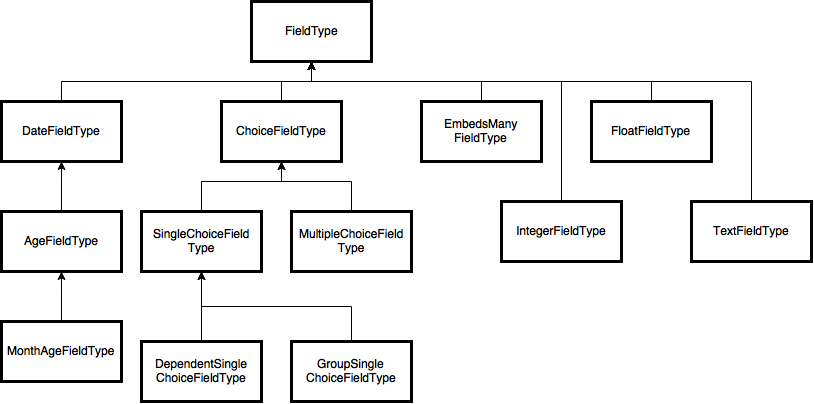
\includegraphics[width=\textwidth]{field_types}
\end{figure}

Eine Herausforderung bilden hier vor Allem die Felder der Klasse ChoiceFieldType. Die anderen Felder können problemlos in eine Flache Struktur überführt werden. Für Choice Felder, sollte nun gemäß der zweiten Normalform (FIX WELCHE NORMALFORM? QUELLE) eine eigene Tabelle mit Relation angelegt werden. Die MultipleChoice Felder müssten weiterhin mit einer `has-many' Relation abgebildet werden, was zu vielen Joins bei Queries führen würde. Da Joins im Allgemeinen verhältnismäßig langsam sind (FIX QUELLE), ist dies in Anbetracht der Aufgabenstellung ein Problem. Da die Datenbank im Microservice jedoch lediglich zu möglichst schnellen Abfrage der Daten, nicht aber zur Pflege und Organisation der Daten genutzt wird, ist es hier vertretbar eine denormalisierte Struktur zu wählen. So entschloss ich mich für den Einsatz von Bitstrings. Jede Auswahlmöglichkeit wird hier durch ein Bit repräsentiert. So kann zum Beipsiel die Mehrfachauswahl von Städten in Berlin, mit den drei Auswahlmöglichkeiten Hamburg, Berlin und München, auf einen drei Bit langen Bitstring abgebildet werden. Der Bitstring `010' in der Datebank bedeutet dann, dass nur die Option Berlin, nicht aber die Optionen Hamburg und München ausgewählt wurden. Dies spart zum Einen Platz in der Datenbank, zum Anderen reduziert es den Einsatz von Datenbankjoins. Es muss natürlich ein Overhead beim Übersetzen der alten Queries in ein Bitstring Format eingeplant werden. Weiterhin wird hier eine Kopplung zwischen Code und Datenbank eingeführt. Wenn sich die Optionen in der Datenbank ändern, muss immer zusätzlich zu allen anderen Stellen diese eine Stelle im Code aktualisiert werden.

Eine weitere Schwierigkeit stellen hier die EmbedsMany Felder dar. Auch hier ist eine `has-many` Relation notwendig, diese kann aber nicht, wie bei sich wiederholenden Auswahlfeldern, durch einen Bitstring ersetzt werden. (FIX MORE STUFF)

Zusätzlich zur relationalen Datenbank setzte ich in der Entwicklung weiterhin Redis\footnote{http://redis.io/} als Zwischenspeicher ein. Redis ist ein in-memory data store, der sowohl zu Datenbankzwecken, als auch zu caching Zwecken genutzt werden kann. Da die Daten ausschließlich im Arbeitsspeicher des Systems abgelegt werden, können hier sehr hohe Geschwindigkeiten erreicht werden.
Zunächst überträgt die Hauptanwendung in Form eines POST requests die Query. Diese wird dann in Redis gespeichert. Die errechneten Queryergebnisse werden dann ebenfalls in Redis gespeichert. Die Ergebnisse können dann jederzeit von der Hauptanwendung abgefragt werden. Außerdem ist es möglich und perspektivisch geplant, die Geschwindigkeit von Redis für das Caching zu nutzen. Es kann überprüft werden ob übertragene Queries bereits bekannt sind und anhand dessen Alters die Ergebnisse übernommen werden. Weiterhin kann hier Performance gewonnen werden, da keine langfristige Persistenz gefordert ist. So kann Redis einzig und allein im Arbeitsspeicher speichern und muss nicht, wie sonst üblich, jede Änderung auf der Festplatte speicher.\footnote{http://redis.io/topics/faq}
Redis speichert Werte grundsätzlich unter einem Stringschlüssel ab. Nach einem Query POST wird hierzu ein kryptischer Schlüssel erzeugt und direkt an die Clientanwendung zurückgegeben. Mit Hilfe der Ruby SecureRandom Bibliothek wird ein 32 Zeichen langer Hexadezimal Schlüssel erzeugt. Somit kann sichergestellt werden, das keine Queries anderer Nutzer ausgelesen werden können, in dem der Schlüssel beabsichtigt verändert wird. Da es keine verschiedenen Zugriffslevel der einzelnen Benutzer gibt, ist es nicht notwendig hier ein ausgefeiltes Authentifizierungssystem einzubauen. Lediglich aus Gründen der Privatsphäre werden hier keine fortlaufenden Schlüssel verwendet.
Damit es jedoch auch nicht zu Kollisionen in der Schlüsselerzeugung kommt, wurde ein ausreichend langer Schlüssel gewählt. Bei einem 32 Zeichen langen Hexadezimal Schlüssel berechnet sich die Anzahl der möglichen Schlüssel wie folgt:
$ t = 16^{32} = 3,4 * 10^{32} $
Selbst nach einer Milliarde generierter Schlüssel ist die Wahrscheinlichkeit von Kollisionsfreiheit demnach noch bei über $99,9999999999999999998$\%.%(FIX QUELLE)
Dies ist eine ausreichend hohe Sicherheit für den Anwendungsfall, zumal die Daten meist nach mehr als einem Tag nicht mehr abgefragt werden.

\subsection{Architektur des Microservices}
%(FIX IS THIS RELEVANT??)
Während der Entwicklung der Anwendung entwickelte ich durchgehend testgetrieben. Da die entwickelte Funktionalität einen integralen Bestandteil der Gesamtanwendung bildet, ist es zwingend notwendig die Funktionalität zu gewährleisten. Um die Qualität der Anwendung zu gewährleisten setzte ich die gleichen Tools ein, die auch in der Hauptanwendung genutzt werden. Als Testframework ist dies RSpec\footnote{http://rspec.info/}. Zur Überprüfung der Code Konventionen wird der Static Code Analyzer RuboCop\footnote{https://github.com/bbatsov/rubocop} eingesetzt. Der Einsatz von RSpec und RuboCop wird sowohl lokal, als auch automatisiert im Continuous Integration System Circle CI\footnote{https://circleci.com} eingesetzt. Fehler der Erfüllung der Fehlerfreiheit bei RSpec und Rubocop führen jeweils zu fehlerhaften Tests. Im eingesetzten Git System Github\footnote{https://github.com} wird bei jedem gepushten Commit automatisch ein Upload zu Circle CI getriggered. Bei Fehlern wird der Branch in Github als rot, ansonsten als grün markiert. Dies ist zwingende Voraussetzung für die den Einsatz von Continuous Deployment.

Wie bereits beschrieben, handelt es sich beim entwickelten Microservice streng genommen lediglich um eine Query Schnittstelle zu einer Datenbank. Der Overhead soll hier möglichst gering gehalten werden. Da in der bestehenden Anwendung möglichst wenig Änderungen vorgenommen werden sollen und die Schnittstelle zur alten Datenbank übergangsweise weiterhin bestehen soll, bietet es sich an, an den Microservice zum Abfragen der Daten die bestehenden Datenbankfelnamen zu übergeben. Die bestehende Schnittstelle zu MongoDB bietet hier eine praktische $.to_json$ Methode mit der ein Query leicht in ein gut übertragbares Format überführt werden kann. Eine erstellte Abfrage auf alle Nutzer die als Sprache deutsch angegeben haben

\begin{lstlisting}[language=Ruby]
User.where(:'profile.basic.locale.value' => 'de')
\end{lstlisting}

\noindent kann so leicht in ein JSON-Format überführt werden:

\begin{lstlisting}[language=Ruby]
User.where(:'profile.basic.locale.value' => 'de').selector.to_json
=> { "profile.basic.locale.value": "de" }
\end{lstlisting}

\noindent So bildet das Übersetzen der übergebenen einen wesentlichen Teil des entwickelten Microservices. (FIX KOPPLUNG erklären und rechtfertigen)

Einen weiteren wesentlichen Bestandteil bildet das handhaben des übergebenen JSON Strings. Dieser wird im ersten Schritt anhand einer JSON Schema\footnote{http://json-schema.org} Definition validiert. So wird sichergestellt das er wohlformattiert ist und den gestellten Anforderungen entspricht. Hier kann vor dem Schritt des wirklichen parsens ggf. noch einmal Last reduziert werden. War die Validierung erfolgreich wird der übergebene JSON String geparsed. Hierzu habe ich einen Parser entwickelt, der das übergeben MongoDB JSON Format in eine PostgreSQL kompatible Notation überführt. Schnell wird jedoch deutlich, dass es weitaus komplexere Querykonstrukte gibt. Da wäre zum Einen der Einsatz von Vergleichsoperatoren. Hier können leicht auch solche Queries entstehen:

\begin{lstlisting}[language=Ruby]
User.where(
    :'profile.basic.locale.value'.nin => ['de', 'de-AT', 'de-CH'],
    :'profile.automotive.car_amount.value'.gt => 3,
    :'profile.automotive.car_amount.value'.lte => 10
).selector.to_json
=> 
{
    "profile.basic.locale.value": {
        "$nin": ["de","de-AT","de-CH"]
    },
    "profile.automotive.car_amount.value": {
        "$gt": 3,
        "$lte": 10
    }
}
\end{lstlisting}

\noindent Dies muss der Parser also auch übersetzen können. Im gleichen Schritt werden, neben dem Parsen, auch die Datenbankfeldnamen übersetzt.

(FIX DEPLOYMENT/Continuous deployment??)
(FIX Funktion?? Was passiert genau im Service? Hier? Wo??)
(FIX Unterpunkte?)
(FIX Testing - how to test Microservices?)

\section{Schaffung einer standardisierten REST Schnittstelle}
Einen entscheidenen Unterschied zwischen Microservice Architektur und monolithischer Entwicklung, bildet die Schnittstelle zwischen den Anwendungsteilen. Während im Monolithen simple code calls stattfinden, muss für die Kommunikation zwischen verschiedenen Servies zunächst ein geeignetes Protokoll zum Austausch gefunden werden.
Da hier eben kein durch die Programmiersprache vorgeschriebener Standard besteht, ist es hier wichtig ein geeignetes Austauschformat zu definieren.
Um Änderungen sowohl im Client, also auch im Service möglich zu machen, sollten keine sprachgebundenen Technologien eingesetzt werden. Somit kann sichergestellt werden, das möglichst geringe Änderungen anfallen, sollte ein neuer Client oder Änderungen am bestehenden System zum Einsatz einer neuen Programmiersprache führen.

Eine populäre Schnittstellentechnologie ist der Einsatz von Remote Procedure Calls (RPC). RPC verfolgt das Hauptziel, remote calls wie lokale Aufrufe wirken zu lassen. Dier ermöglicht es schnell Server-Client Anwendungen zu entwickeln. Zwar sind RPC Lösungen häufig technologiegebunden, es gibt jedoch auch diverse Lösungen die verschiedene Technologien unterstützen. Ein großer Nachteil von RPC wird jedoch bei komplexeren Anwendungen auffällig: Remote Calls sind keine Localaufrufe.~\footcite[][Seite 47]{newman2015building} Zwar erlaubt RPC es durch ``verstecken'' der Implementierungsdetails, schnell einfache Client-Server Anwendungen zu entwickeln, mit der Zeit wird aber deutlich, dass mitunter feinere Entwicklungsmöglichkeiten notwendig sind. Hier fehlt es dann oft an besserer technologischer Kontrolle.

Eine Alternative zu RPC, die vor Allem in den letzten Jahren an Popularität gewonnen hat, ist der Representational State Transfer (REST). Im Gegensatz zu RPC, das ursprünglich für Verteilte Systeme innerhalb eines Netzwerkes oder Netzwerkverbundes entwickelt wurde, ist REST eng an das Internet gekoppelt. Nicht zuletzt deswegen wird REST, trotz relativer Protokollunabhängigkeit, meist mit dem Hypertext Transfer Protocol (HTTP) verwendet. Die prominenten HTTP Verben POST, GET, PUT und DELETE lassen sich direkt zu den CRUD Operationen Create, Read, Update und Delete übersetzten. Eine REST Grundlage stellt die methodische Unabhängigkeit von Resourcen dar. Methoden sollten sich auf allen Resourcen gleich verhalten. So kann mit Hilfe der HTTP Verben durch verschiedene Request auf eine Resource, unterschiedliche Handlungen abgebidet werden. Statt die Methoden $createResourceX$, $readResourceX$, $updateResourceX$ und $deleteResourceX$ zu unterscheiden, kann eine einfache und abstrakte Form der Form $VERB RESOURCE$ genutzt werden um alle Methoden abzubilden. So können Methoden auf Queries also durch simple HTTP Request wie $POST /queries$ und $GET /queries$ abgebildet werden. Ein weiterer Vorteil der relativen Nähe zu HTTP, ist gute Unterstützung dieser Technolgie. Viele Technoligien die mit HTTP zum Einsatz kommen, wie z.B. Caching und Load Balancing, können leicht auch mit REST eingesetzt werden.

Weiterhin ist REST in der Wahl des eingesetzten Austauschformats frei. Populäre Möglichkeiten sind hier z.B. JSON oder XML.

(FIX QUELLEN!!)

(FIX JSON SCHEMA, RAML, Link to RAML doku page, console)

\section{Integration des Microservices in den Monolithen}
Wie bereits im vorangegangenen Kapitel beschrieben, beschloss ich mich die neue Microservice Anwendung mit Hilfe des Flipper Gems parallel zu betreiben. Anhand der abstrahierten Schnittstelle des QueryExecuters, wird entschieden ob ein Query auf der alten Datenbank oder dem neuen Service stattfindet. Das entsprechende Klassendiagramm ist in \autoref{fig:class} dargestellt.
\begin{figure}[!ht]
    \centering
    \caption{Klassendiagramm zur Verteilung zwischen bestehendem und neu geschaffenem Code}
    \label{fig:class}
    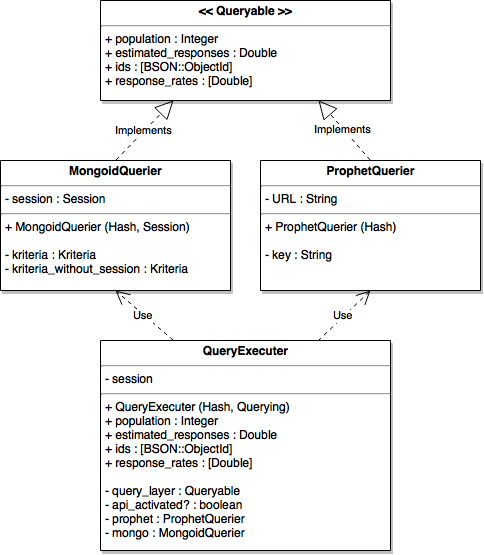
\includegraphics[scale=0.6]{klassendiagramm}
\end{figure}

Ist der Flipper aktiviert, wird zunächst per POST ein Query an den Service übertragen. Im Hintergrund initiiert der Service dann ein parsen, übersetzen und abarbeiten der Query, dies geschieht asynchron. Zunächst wird die Query in Redis gespeichert und der generierte Zugriffsschlüssel zurückgegeben.
Anhand dieses Schlüssels kann die Hauptanwendung dann die freigegebenen Ergebnisse des Querys, wie die Ids der zutreffenden User, abfragen. Der Ablauf kann wie in \autoref{fig:sequenz} visualisiert werden.

\begin{figure}[!ht]
    \centering
    \caption{Sequenzdiagramm zum Profilqueryen bei aktiviertem Flipper}
    \label{fig:sequenz}
    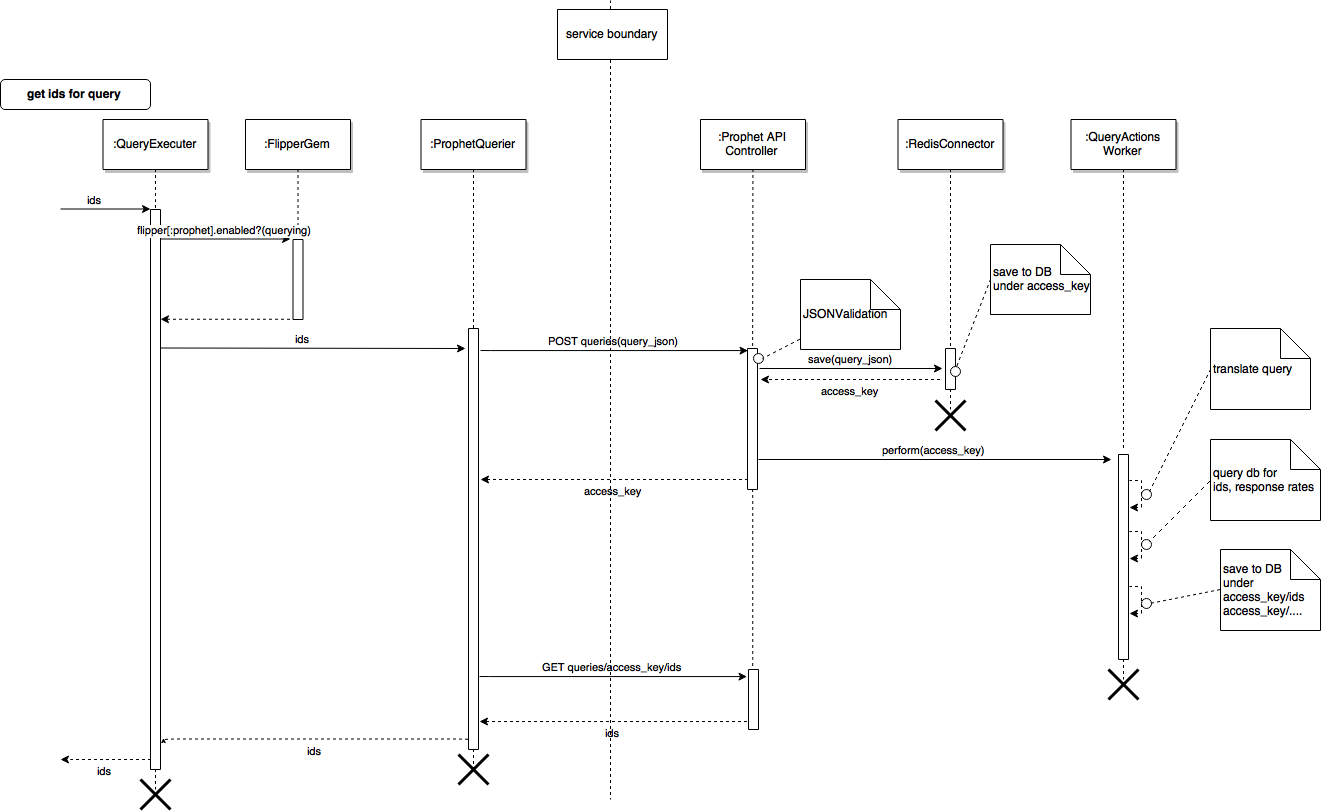
\includegraphics[width=\textwidth]{prophet_sequenz}
\end{figure}

\section{Betrieb der Anwendung auf AWS - Betreuung, Monitoring und Scaling}
Wie bereits beschrieben, bilden die Skalierungsmöglichkeiten von Microservices einen großen Vorteil des Architekturstils. Um diesen optimal ausnutzen zu können, bietet es sich an ein dynamisches Hosting einzurichten. Hier gibt diverse Lösungen, die alle einen ähnlichen Funktionsumfang bieten. Zu nennen sind hier insbesondere Amazon Web Services (AWS), Google App Engine\footnote{https://cloud.google.com/appengine/} und Heroku\footnote{https://heroku.com/}. Da AWS eine der reifsten Platformen ist und ich mit ihr bereits Erfahrunden sammeln konnte, beschloss ich für den Microservice AWS als Hoster zu wählen.
Auf AWS nutze ich Amazon Beanstalk zum Betreiben der Anwendung. Beanstalk nutzt intern EC2 Instanzen, baut aber eine eigene Konfigurationsschicht darauf auf. Daher muss keine gesamte virtuelle Maschine betrieben werden, stattdessen kann die Anwendung leicht über ein Konfigurationsinterface, wie in \autoref{fig:awsui} dargestellt, gesteuert werden.

\begin{figure}[!ht]
    \centering
    \caption{AWS Beanstalk Konfigurationsinterface}
    \label{fig:awsui}
    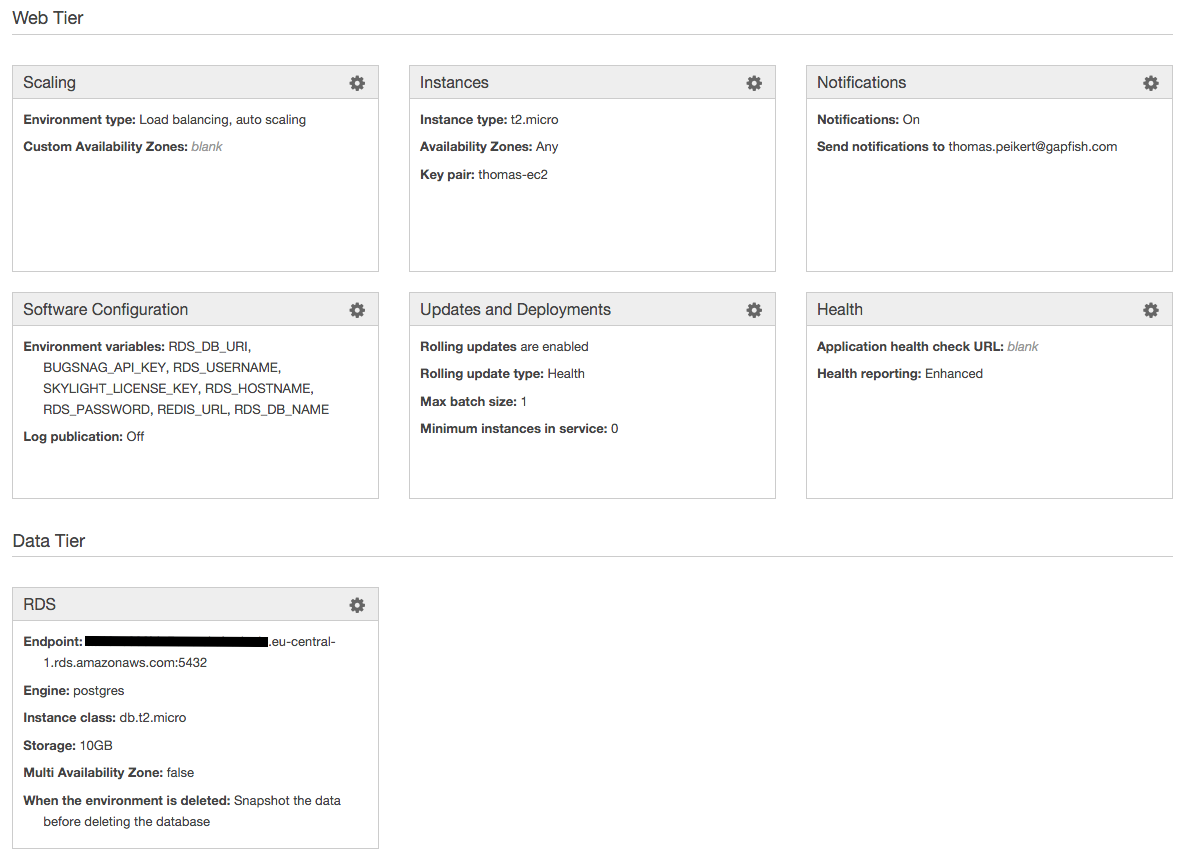
\includegraphics[width=\textwidth]{aws_config_ui}
\end{figure}
AWS Beanstalk ist selbst mit keinen Kosten verbunden, die Kosten ergeben sich ausschließlich aus den von Beanstalk genutzten Resourcen, also die genutzten EC2 Instanzen und der reine Speicherverbrauch der Anwendung auf AWS S3. Die weiteren von der Anwendung benötigten Resourcen sind zum Einen eine PostgreSQL Datenbank und der Key-Value Store Redis. Hierfür bietet Amazon jeweils gesonderte Services zum Betrieb. Relationale Datenbanken können über den Amazon Relational Database Service (RDS) genutzt werden, Redis wird über Amazon ElastiCache angeboten. Beide Services bieten ebenso wie Beanstalk gute Skalierungsmöglichkeiten.

Bisher wurden die gesamte Firmenanwendung auf einem System, bei einem Hoster betrieben. Zwar gibt es durchaus separate Repositories um eine API für die mobilen Anwendungen zu bieten, diese werden jedoch immer über das Ruby Webserver Interface in die bestehende Anwendung eingebunden. So werden sie bei jedem Deploy der Hauptanwendung ebenfalls deployt. Weiterhin laufen sie im selben Prozess auf dem gleichen Server wie die Hauptanwendung. Hier ist also keinerlei separates Handling zum Monitoring notwendig. Es kann auch keinen Ausfall eines Teilsystems geben, da alle Teile zusammenhängen. Lediglich die Datenbanken und Redis laufen auf dedizierten Servern, diese werden aber im gleichen Netzwerk betrieben, somit sind zwar Teilausfälle möglich, diese werden durch ein Primary-Secondary System abgesichert, Netzwerkprobleme sind aber in der Regel ausgeschlossen. Das gesamte System kann wie in \autoref{fig:deployd} dargestellt werden.

\begin{figure}[!ht]
    \centering
    \caption{Deploymentdiagramm: Zusammenspiel aller Komponenten}
    \label{fig:deployd}
    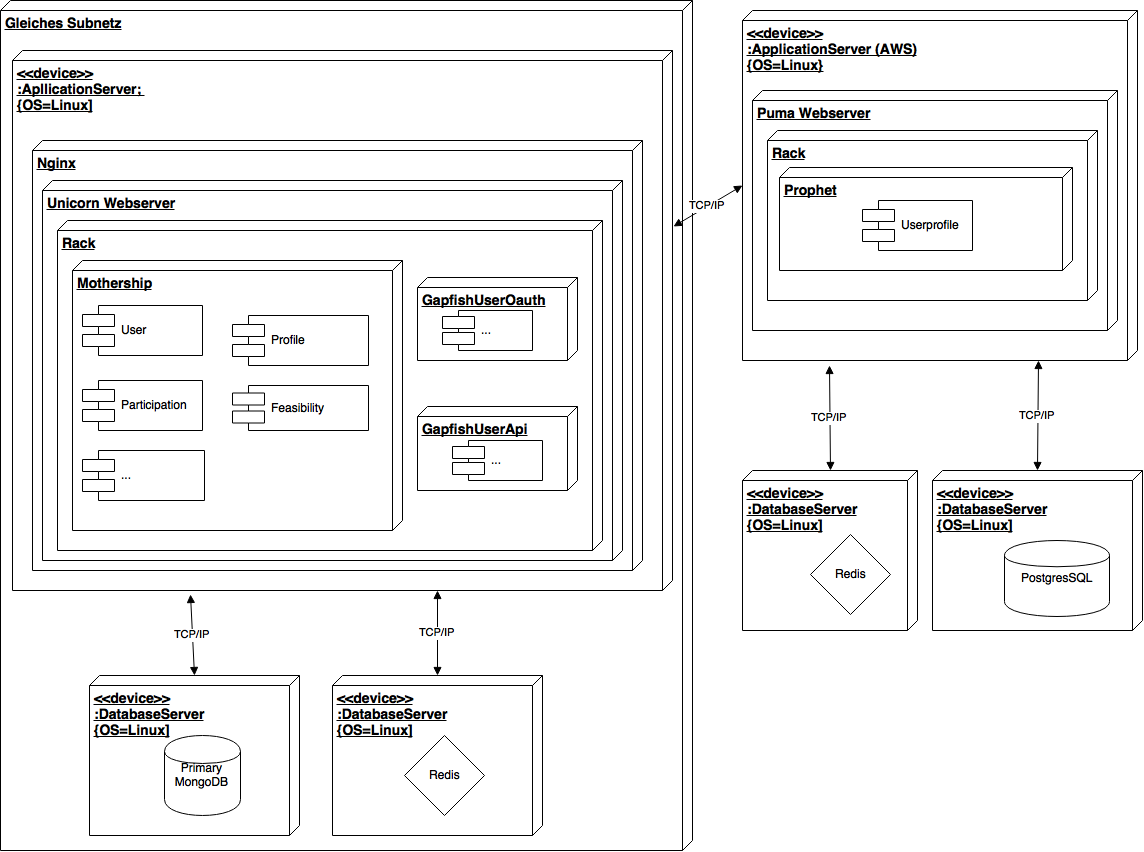
\includegraphics[width=\textwidth]{deploymentdiagram}
\end{figure}

Besonders wichtig für den Microservice ist daher das Monitoring der Anwendung und des Servers. Da hier ein von der Hauptanwendung komplett separates System betrieben wird, muss hier sichergestellt werden, dass zum Einen Fehler schnell erkannt und zum Anderen schnell behoben werden. 

Zum Monitoring nutze ich zum Einen Amazons eigene Monitoring Lösung, die über den Gesundheitsstatus der Anwendung informiert. Wechselt die Anwendung vom Gesundheitsstatus ``OK'' in einen anderen, werden die Entwickler direkt über eine Email informiert.

Zusätzlich zum allgemeinen Ausfallmonitoring durch Amazon, integrierte ich das Monitoring Tool Skylight\footnote{https://www.skylight.io/} in die Anwendung. Im bisherigen Betriebssetup wird aktuell NewRelic\footnote{http://newrelic.com/} zum Monitoring eingesetzt. Skylight zeichnet sich jedoch durch einen besonders geringen Overhead aus, was sich beim Microservice durchaus anbietet. Skylight informiert ebenfalls per Email über Ausfälle und zeichnet allgemein die Performance des Systems auf. So kann zu jedem Zeitpunkt der Vergangenheit, über Wochen hinweg, detailliert die Performance des Sytsems nachvollzogen werden. Zusätzlich zu allgemeinen Aufzeichnungen der Response time, kann hier nach Datenbankabfragen unterschieden werden. So wird schnell deutlich, welche Anfragen besonders zeitintensiv sind und wo Handlungsbedarf oder Verbesserungsmöglichkeiten bestehen. 

Als Fehlerreporting Tool kommt im Microservice Bugsnag\footnote{https://bugsnag.com} zum Einsatz. Bugsnag wird bereits als primäres Firmentool verwendet und eignet sich ebenfalls gut für kleine Anwendungen. Bugsnag zeichnet Fehler im System mit Stacktrace auf und informiert die Entwickler ebenfalls per Email.

Das informieren über Fehler per Email ist im Betrieb ein durchaus üblicher Weg, daher eignet sich diese Integration auch für den neuen Service. Weiterhin besteht in der Firma ein Dashboard, was zwar nicht die Performance des neuen Microservices an sich, aber die Gesamtperformance des Sampling Prozesses darstellt. Dieser umschließt alles vom Erstellen der Query, der Abfrage des neuen Services, bis hin zum verarbeiten und anzeigen der Queryergebnisse. So können Probleme auf dem Dashboard leicht von den Entwicklern bemerkt werden. All dies sind im Live Betrieb erprobte Techniken und eignen sich dadurch sehr gut für die Ausweitung auf neue Services.